\chapter{Vergleich und Bewertung zwischen Open API 2.0 und Open API 3.0}
\label{cha:k6}
Ende 2017 wurde die Open API Specification 3.0 schließlich von der Open API Initiative veröffentlicht. Es ist eine Hauptversion und nach 3 Jahren hat es eine Menge Verbesserungen gegenüber der Open API 2.0-Spezifikation gebracht, sodass Definitionen für eine breitere Palette von APIs erstellt werden können. In diesem Kapitel werden die Hauptunterschiede zwischen Open API 2.0 und 3.0 nach der Quellen\cite{swagger20Github, openapi20Github} aufgezeigt, um ein Wegweiser für die Entwicklung des Open API 3.0 Plugins für das Open Source Werkzeug OWASP Zap zu sein.

\section{Strukturelle Verbesserungen}

Mit der OpenAPI Specification Version 3.0 wurde die Gesamtstruktur des Dokuments vereinfacht:

\newpage

\begin{figure}[h]
	\centering
	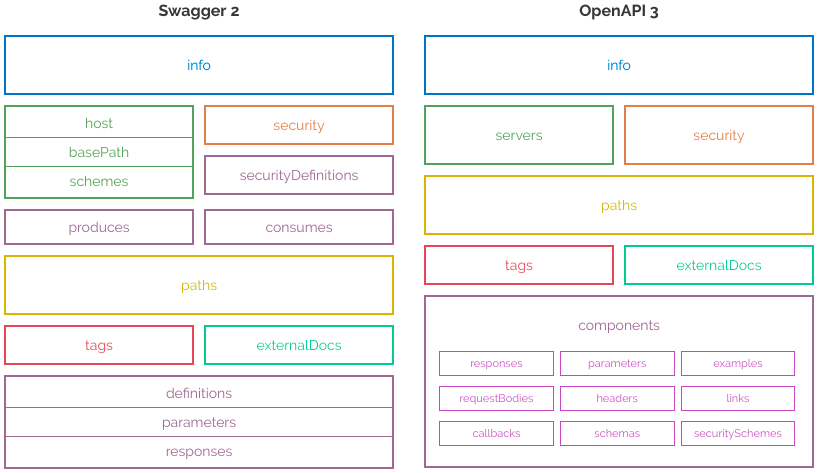
\includegraphics[width=12cm]{openapi2u3.png}
	\caption{Überblick über die Struktur der Open API 2.0 und Open API 3.0 Spezifikationen\cite{openapi2u317}}
	\label{openapi2u317-1}
\end{figure}

\subsection{Versionsbezeichner (engl. Version Identifier)}

Version ist eine beliebige Zeichenfolge, die die Version von API angibt\cite{openapiversion17}. In 2.0 spec gibt es eine Eigenschaft namens "`swagger"', die die Version der Spezifikation angibt, zum Beispiel:\\

\begin{LaTeXCode}[caption={Version von Swagger},captionpos=b, label=LaTeXCode:swagger2.0-1][numbers=none]
"swagger": "2.0"\\
\end{LaTeXCode}

Die Versionseigenschaft, die von 2.0 als Swagger bezeichnet wurde, wird in Version 3.0 durch eine Versionskennung von Open API ersetzt.\\

\begin{LaTeXCode}[caption={Version von Open API},captionpos=b, label=LaTeXCode:openapi3.0-1][numbers=none]
"openapi": "3.0.0"\\
\end{LaTeXCode}

\subsection{Komponenten (engl. Components)}

Oft haben mehrere API-Operationen einige gemeinsame Parameter oder geben dieselbe Antwortstruktur zurück. Um Code-Duplizierungen zu vermeiden, kann die allgemeinen Definitionen in den Abschnitt für globale Komponenten eingefügt werden und mit \texttt{\$ref} referenziert werden. Komponenten dienen als Container für verschiedene wiederverwendbare Definitionen. Die Definitionen in Komponenten haben keine direkten Auswirkungen auf die API\cite{openapicomponents17}.\\

Swagger 2.0 enthält separate Abschnitte für wiederverwendbare Komponenten wie z.B. \texttt{"`definitions"'}, \texttt{"`parameters"'}, \texttt{"`responses"'} und \texttt{"`securityDefinitions"'}.\\

\begin{LaTeXCode}[caption={Open API 2.0 - Komponenten\cite{openapicomponents17}},captionpos=b, label=LaTeXCode:openapi3.0-2][numbers=none]
// Swagger 2.0    

'#/definitions/User'
'#/parameters/offsetParam'
'#/responses/ErrorResponse'
\end{LaTeXCode}

In OpenAPI 3.0 wurden sie alle in Komponenten verschoben. Außerdem wurden Definitionen als Schemas umbenannt und securityDefinitions als securitySchemes umbenannt.\\

\begin{LaTeXCode}[caption={Open API 3.0 - Komponenten\cite{openapicomponents17}},captionpos=b, label=LaTeXCode:openapi3.0-3][numbers=none]
// OpenAPI 3.0

'#/components/schemas/User'
'#/components/parameters/offsetParam'
'#/components/responses/ErrorResponse'
\end{LaTeXCode}

Swagger 2.0 hat das Konzept der Definitionen, sie sind jedoch etwas inkonsistent und sind nicht so klar definiert. OpenAPI 3.0 versucht, das Konzept in Komponenten zu standardisieren, bei denen es sich um definierbare Objekte handelt, die an mehreren Stellen wiederverwendet werden können. Wenn für mehrere Operationen einer API eine ähnliche Eingabestruktur erforderlich ist, kann die Eingabestruktur unter der Komponente als Anforderungstext definiert und in mehreren Pfaden wiederverwendet werden. Ebenso können Header, Antworten usw. auch wiederverwendet werden. Dies ist wichtig, da dadurch einige wesentliche Wiederverwendungsvorteile hinzugefügt werden, die in Version 2.0 nicht möglich sind.\\

\subsubsection{Anfrage-Format (engl. Request Format)}

Anfrage-Body wird in der Regel für "`Erstellen"' und "`Aktualisieren"' von Operationen (\texttt{POST}, \texttt{PUT}, \texttt{PATCH}) verwendet. Wenn eine Ressource mit \texttt{POST} oder \texttt{PUT} erstellt wird, enthält der Anforderungshauptteil normalerweise die Darstellung der Ressource, die erstellt werden soll\cite{openapirequestbody17}.\\

Einer der verwirrendsten Aspekte von Swagger 2 war \texttt{body/formData}.

\begin{LaTeXCode}[caption={Swagger 2.0 - Anfrage-Format},captionpos=b, label=LaTeXCode:openapi3.0-4][numbers=none]
"/examples/{exampleId}":
post:
parameters:
- name: exampleId
in: path
description: identification number of example to update
required: true
type: string
- name: user example
in: body
description: user example to add to the database
required: true
schema:
type: array
items:
type: string
\end{LaTeXCode}

Bei dem OpenAPI 3.0 wird \texttt{body} in seinen eigenen Abschnitt mit dem Namen \texttt{requestBody} verschoben und \texttt{formData} wurde darin zusammengeführt. Zusätzlich wurden Cookies als Parametertyp hinzugefügt.

\begin{LaTeXCode}[caption={Open API 3.0 - Anfrage-Format},captionpos=b, label=LaTeXCode:openapi3.0-5][numbers=none]
"/examples/{exampleId}":
post:
	requestBody:
		description: user example to add to the database
		required: true
		content:
			application/json: 
			 schema:
			  type: array
			  items:
			   \$ref: '#/components/schemas/Example'
			examples:
			 - name: Example
			   exampleType: Example Type
			 - http://example.com/example.json
	parameters:
	 - name: exampleId
	 in: path
	 description: identification number of example to update
	 required: true
	 type: string
\end{LaTeXCode}

Der \texttt{requestBody} hat viele neue Funktionen. Man kann jetzt ein Beispiel (oder ein List von Beispielen) für \texttt{requestBody} angeben. Dies ist ziemlich flexibel (Man kann dem Beispiel ein vollständiges Beispiel, eine Referenz oder sogar eine URL übergeben).

Der neue \texttt{requestBody} unterstützt verschiedene Medientypen (Inhalt ist ein Array von Mimetypen wie \texttt{application/json} oder \texttt{text/plain}).

\subsubsection{Antwort-Format (engl. Response Format)}

Eine API-Spezifikation muss die Antworten für alle API-Vorgänge angeben. Für jede Operation muss mindestens eine Antwort definiert sein, normalerweise eine erfolgreiche Antwort. Eine Antwort wird durch ihren HTTP-Statuscode definiert und die Daten werden im \texttt{response body} oder in den Kopfzeilen zurückgegeben. Bei den Antworten beginnt jede Antwortdefinition mit einem Statuscode, z. B. 200 oder 404. Eine Operation gibt normalerweise einen erfolgreichen Statuscode und einen oder mehrere Fehlerstatus zurück\cite{openapiresponsebody17}.

Bei dem OpenAPI 3.0 werden auch Antwort-Format aktualisiert. Man kann jetzt eine Antwort wie bei dem Quelcode \ref{LaTeXCode:openapi3.0-6} definieren, anstatt jede separat definieren zu müssen.

\begin{LaTeXCode}[caption={Open API 3.0 - Antwort-Format},captionpos=b, label=LaTeXCode:openapi3.0-6][numbers=none]
myExample:
	'\$request.body#/url':
	post:
		requestBody:
		  description: Response example
	    content:
		  'application/json':
		    schema:
			  \$ref: '#/components/schemas/ResExample'
			responses:
			  200:
			  description: response works!
\end{LaTeXCode}


\subsubsection{Verlinkung (engl. Linking)}

Mit Links können Sie beschreiben, wie verschiedene Werte, die von einer Operation zurückgegeben werden, als Eingabe für andere Operationen verwendet werden können\cite{openapilinks17}.

OpenAPI 3.0 Spezifikation unterstützt das Verknüpfen, sodass Beziehungen zwischen Pfaden sauber beschrieben werden können und diese Version bisher am widerstandsfähigsten macht. Angenommen, dass es einen Benutzer erhielt wird und er hat ein Id. Dieses Id ist an sich ziemlich nutzlos. Man kann Verlinkungen verwenden, um zu zeigen, wie man dieses Id erweitern und die vollständige Adresse erhalten.

\begin{LaTeXCode}[caption={Open API 3.0 - Verlinkungen},captionpos=b, label=LaTeXCode:openapi3.0-7][numbers=none]
paths: 
	/users/{userId}:
	 get:
	  responses:
	   200:
	    links:
	     address:
	      operationId: getExampleWithId
		  parameters:
		   exampleId: '\$response.body#/exampleId'
\end{LaTeXCode}

Wie bei dem Quellcode \ref{LaTeXCode:openapi3.0-7} gesehen, dass in der Antwort von \texttt{/users/{userId}} eine \texttt{exampleId} zurück erhält. Die Verlinkung beschreibt, wie man das \texttt{Example} erhält, indem man auf \texttt{\$response.body\#/exampleId} verweist.

\subsubsection{Rückrufe (engl. Callbacks)}

Bei dem OpenAPI 3.0 können jetzt Rückrufe wie bei dem Quelcode \ref{LaTeXCode:openapi3.0-10} definiert werden. Das heißt, dass asynchrone Anforderungen, die die Dienste als Reaktion auf bestimmte Ereignisse an einen anderen Dienst gesendet werden. Auf diese Weise können die Workflows verbessert werden, die die API die Clients bietet. Ein typisches Beispiel für einen Rückruf ist eine Abonnementfunktionalität (engl. Subscription). Benutzer abonnieren bestimmte Ereignisse des Dienstes und erhalten eine Benachrichtigung, wenn dieses oder jenes Ereignis eintritt. Beispielsweise kann ein E-Shop bei jedem Einkauf eine Benachrichtigung an den Manager senden\cite{openapicallbacks17}.

\begin{LaTeXCode}[caption={Open API 3.0 - Callbacks\cite{openapicallbacks17}},captionpos=b, label=LaTeXCode:openapi3.0-10][numbers=none]
POST /subscribe
Host: my.webpage.com
Content-Type: application/json
{
	"callbackUrl": "https://myserver.com/send/callback/here"
}
\end{LaTeXCode}

Diese Beschreibung vereinfacht die Kommunikation zwischen verschiedenen Servern und hilft der Verwendung von Callbacks in der API zu standardisieren.

\subsection{Servers}

Der Abschnitt "`Server"' gibt den API-Server und die Basis-URL (Base URL) an. Es kann einen oder mehrere Server definiert werden, z. B. Produktion und Sandbox\cite{openapiserver17}. Alle API-Endpunkte sind relativ zur Basis-URL. Angenommen, die Basis-URL von \texttt{https://api.example.com/v1}. Der Endpunkt \texttt{/users} verweist beispielsweise auf \texttt{https://api.example.com/v1/users}\cite{openapiapiserverundbaseurl17}.\\

Bei der Beschreibung der API kann jetzt mehrere Hosts bereitgestellt werden, sodass besser mit der Komplexität umgehen werden können, wie sich APIs an einem einzelnen Standort befinden oder sich auf mehrere Cloud-Standorte und die globale Infrastruktur verteilen. Derzeit kann mit Swagger 2 \texttt{schemes}, \texttt{host} und \texttt{baseUrl} wie bei dem Quellcode \ref{LaTeXCode:openapi3.0-8} definiert werden, die in der URL zusammengefasst sind. 

\begin{LaTeXCode}[caption={Swagger 2.0 - Server},captionpos=b, label=LaTeXCode:openapi3.0-8][numbers=none]
info:  
	title: Swagger Example
host: example.com  
basePath: /v1  
schemes: ['http', 'https']
\end{LaTeXCode}

Mit OpenAPI 3.0 können jetzt mehrere URLs haben (siehe Quellcode \ref{LaTeXCode:openapi3.0-9}), die beliebig definiert werden können. Das bedeutet, dass wie zuvor nur einen an der Basis haben können oder ein bestimmter Endpunkt kann einen eigenen Server haben, wenn die Basis-URL unterschiedlich ist. Darüber hinaus ist das Templating von Pfaden jetzt zulässig.

\begin{LaTeXCode}[caption={OpenAPI 3.0 - Server},captionpos=b, label=LaTeXCode:openapi3.0-9][numbers=none]
servers:  
- url: https://example.com/{version}
	description: The main prod server
	variables:
	  subdomain:
	   default: production
	  version:
	   enum:
		- v1
		- v2
	   default: v2
\end{LaTeXCode} 

\subsection{Ausbau des JSON Schema Supports}

OpenAPI 3.0 bietet mehrere Schlüsselwörter, mit denen die Schemas kombiniert werden können. Mit diesen Schlüsselwörtern kann ein komplexes Schema erstellt werden oder einen Wert anhand mehrerer Kriterien überprüft werden\cite{openapijsonaufbau17}:

\begin{itemize}
	\item \texttt{oneOf}: validiert den Wert anhand genau eines der Subschemas
	\item \texttt{allOf}: validiert den Wert anhand aller Unterschemas
	\item \texttt{anyOf}: validiert den Wert anhand eines (eines oder mehrerer) der Subschemas
\end{itemize}

\begin{LaTeXCode}[caption={OpenAPI 3.0 - JSON Schema Supports Beispiel},captionpos=b, label=LaTeXCode:openapi3.0-11][numbers=none]
paths:
	/pets:
	  patch:
 		requestBody:
		  content:
		    application/json:
			  schema:
			    oneOf:
				  - $ref: '#/components/schemas/Cat'
				  - $ref: '#/components/schemas/Dog'
		responses:
		  '200':
		    description: Updated
\end{LaTeXCode} 

Quellcode \ref{LaTeXCode:openapi3.0-11} zeigt, wie das \texttt{Request body} in der Aktualisierungsoperation überprüft wird. Es wird verwendet werden, um zu überprüfen, dass das \texttt{Request body} alle erforderlichen Informationen zu dem zu aktualisierenden Objekt enthält, abhängig vom Objekttyp.

\subsection{Beispiele Objekt (engl. Examples Object)}

Parametern, Eigenschaften und Objekten Beispiele hinzugefügt werden, um die OpenAPI-Spezifikation des Web-Service klarer zu machen. Beispiele können von Tools und Bibliotheken gelesen werden, die die API auf irgendeine Weise verarbeiten. Ein API-Mocking-Tool kann beispielsweise Beispielwerte verwenden, um \texttt{Mock-Request} zu generieren\cite{openapiexample17}.

\begin{LaTeXCode}[caption={OpenAPI 3.0 - Examples Object Beispiel},captionpos=b, label=LaTeXCode:openapi3.0-12][numbers=none]
paths:
	/users:
	  post:
		summary: Adds a new object
		requestBody:
		  content:
		    application/json:
		      schema:
			    \$ref: '#/components/schemas/Object'
			  example:
			    id: 10
			    name: Object Example
		responses:
	      '200':
		    description: OK
\end{LaTeXCode}

Bei dem OpenAPI 3.0 wurden die Möglichkeiten zur Beschreibung von Beispielen erheblich erweitert. In der vorherigen Spezifikation (Swagger 2.0) wurde angegeben, dass Beispiele nur von einem JSON- oder YAML-Objekt beschrieben werden können. Bei dem OpenAPI 3.0  kann nun durch Verwendung einer \texttt{json string} jedes Beispielformat beschrieben werden. Darüber hinaus kann ein \texttt{\$ref}-Objekt verwendet werden, um auf externe Dateien mit Beispielen zu verweisen.

\subsection{Sicherheit (engl. Security)}

Die Sicherheit wird anhand der Schlüsselwörter \texttt{securitySchemes} und \texttt{security} beschrieben. Es werden mit securitySchemes alle Sicherheitsschemata definiert, die die API unterstützt und wird die Sicherheit verwendet, um bestimmte Schemas auf die gesamte API oder einzelne Vorgänge anzuwenden\cite{openapisecurity17}: 

\begin{LaTeXCode}[caption={OpenAPI 3.0 - Security},captionpos=b, label=LaTeXCode:openapi3.0-13][numbers=none]
components:  
	securitySchemes:
		UserSecurity:
		  type: http
		  scheme: basic
		APIKey:
		  type: http
		  scheme: bearer
		  bearerFormat: TOKEN
\end{LaTeXCode}

Bei dem OpenAPI 3.0 wurde \texttt{securityDefinitions} (siehe \ref{LaTeXCode:openapi3.0-13}) als \texttt{securitySchemes} umbenannt und in den \texttt{Components} verschoben. Außerdem ist \texttt{http} ein übergeordneter Typ für alle \texttt{HTTP security scheme} wie z.B. \texttt{basic}, \texttt{bearer} und \texttt{other}. Des Weitreren gibt das Schlüsselwort \texttt{schema} den Schematyp an.






















